\chapter{Investeren en Handelen}
\label{ch:investing}

Dit hoofdstuk behandelt de basis van twee verschillende strategie\"en die worden ingezet om doelen te bereiken - beleggen en investeren versus handelen en traden in cryptocurrency. Zowel beleggers als handelaren proberen winst te maken door middel van markt-participatie, maar het zijn twee zeer verschillende methoden om winst te maken. 

    \medskip
    \begin{quotation}
          \textit{\say{Investing and trading is all about opportunities and probabilities, rather than certainties}}
          \begin{flushright}
            \small{--- \textbf{Cryptomanuals}}
          \end{flushright}
    \end{quotation}
       \medskip
   

\section{Investeren en beleggen}
Investeren is het vastleggen van kapitaal in een project of een onderneming, om winst te maken of het project te steunen. Het kan naast crypto ook in een individueel aandeel zijn, een beleggingsfonds, een onroerend goed, of iets anders dat vandaag minder waarde heeft dan het in de toekomst geacht wordt te hebben. 

    \medskip
    \begin{cryptobox}{LANGE TERMIJN}
        Beleggen - een lange termijninvestering - is voornamelijk interessant omdat de re\"ele waarde van een investering over een langere periode wordt gecre\"eerd en men de investeringen kan opvolgen en zien groeien. Beleggen is dus investeren in de toekomst, en met geld dat niet direct nodig is om lopende kosten te dekken of spullen aan te schaffen.
    \end{cryptobox}
    \medskip
    
Investeer alleen in projecten waarvan je hebt vastgesteld dat ze potentieel hebben of handel op basis van een goede technische analyse of andere onderzoeksinspanningen, zie daarvoor \cref{ch:research}.

\subsection*{Waarom investeren?}
Het doel van beleggen is het geleidelijk opbouwen van vermogen over een langere periode door middel van het kopen en houden van een portefeuille van aandelen, beleggingsfondsen, obligaties en andere beleggingsinstrumenten. Beleggers vergroten vaak hun winst door eventuele winsten te herinvesteren. Beleggers houden vaak jarenlang of zelfs decennialang beleggingen aan, waarbij ze in bepaalde gevallen kunnen profiteren van extra's zoals (samengestelde) rente en dividend.

\section{Handelen}
Cryptocurrency handelaren (traders) willen profiteren van korte termijn schommelingen in prijs. Traders kunnen profiteren van zowel stijgende als dalende markten om posities te betreden en te verlaten over een kortere periode, waardoor kleinere - meer frequente - winsten worden gemaakt. Als je een handelaar bent, dan ben je een persoon die (vele) transacties cre\"eert. Je koopt of verkoopt de investeringen op relatief korte termijn, op verschillende prijsniveaus.

   \medskip
    \begin{cryptobox}{KORTE TERMIJN}
       Cryptocurrency handelaren speculeren op toekomstige koersveranderingen op basis van historische gegevens en patronen. Hierbij minimaliseren zij het risico met behulp van technische hulpmiddelen en expertise. Het handelen in cryptocurrency kan zeer stressvol zijn, juist door de hoge snelheid waarmee de prijzen fluctueren. Binnen de cryptocurrencymarkt valt voor handelaren vrijwel altijd wat te verdienen, ook in een markt waarbij de koersen al geruime tijd dalen.
    \end{cryptobox}
    \medskip

Cryptocurrency handelaren kunnen crypto kopen zonder enige persoonlijke connectie met het eigenlijke product of de eigenlijke dienst - ze kijken alleen maar naar posities met winstmarges, ongeacht het doel van het project zelf. Daarom kijken ze niet naar fundamentele eigenschappen, omdat ze kunnen profiteren van de (snel) wisselende koers binnen fracties van minuten, uren of dagen. 

\begin{figure}
    \centering
    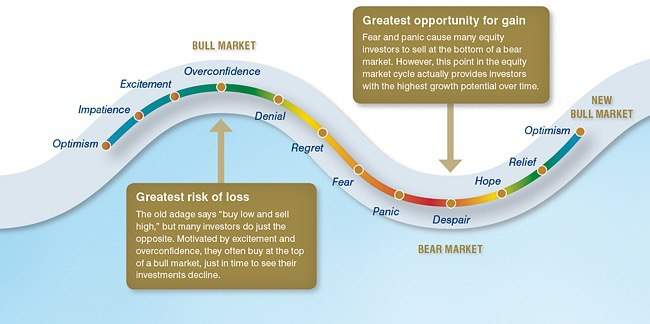
\includegraphics[width=.95\textwidth]{img/ch-investing/bear_bullmarket.jpg}
    \caption[Bear and bull markets and market psychology]{Marktpsychologie is grotendeels de drijvende kracht achter de  \say{bear} en \say{bull} markt. In elke fase van de emotionele cyclus zijn er beslissingen te nemen door investeerders.}
    \label{fig:bear_bullmarket}
    \source{Brightscope; \href{https://www.brightscope.com/financial-planning/advice/article/30367/Breaking-The-Emotional-Cycle-Of-Investing}{Research and Data}.}
\end{figure}
    
    
\section{Aandachtspunten}
Wanneer men zich na eigen onderzoek veilig voelt bij een investering of trade, kan men kijken naar de \say{optimal entry points}, het beste moment om in te stappen. Dit doe je door naar de historische prijsniveaus te kijken in verhouding tot de huidige prijs. Dit kan op platforms zoals \href{https://www.coinigy.com/?r=17fa0d35}{Coinigy} of \href{https://www.tradingview.com/}{TradingView}. Kijk voor meer informatie over technische analyse in \cref{sec:technicalanalysis}. Bij het kiezen voor een lange termijn investering of een korte termijn trade, horen ook verschillende aanpakken en strategie\"en, die hierna worden besproken.

\subsection{Aanpak investeren}
 Beleggers en investeerders kijken niet elke dag naar de koers, maar richten zich liever op de horizon, waar de koers heen gaat.
 In het algemeen streven lange termijn beleggers naar een hoger rendement over een langere periode. Terwijl de koersen onvermijdelijk schommelen, zullen beleggers de dalende trend veelal uitzitten met de verwachting dat de prijzen weer zullen stijgen en eventuele verliezen die je hebt geleden uiteindelijk zullen herstellen. Beleggers zijn doorgaans meer bezig met de fundamentele eigenschappen van de verschillende beleggingen, zoals bedrijfs-prognoses, toekomstplannen, de kwaliteit van het achterliggende team en het probleem dat aangepakt wordt. Dat de koers ook wel eens door een dal gaat is daarbij niet meer dan normaal. 

    \begin{quotation}
        \textit{\say{Stake it till you make it.}}
            \begin{flushright}
                \small{--- \textbf{Cryptomanuals}}
            \end{flushright}
    \end{quotation}

\paragraph{Aandachtspunten} 

\begin{enumerate}[label=(\alph*)]
  \setlength\itemsep{0em}
    \item \textbf{Fundamental research}. Onderzoek het project en het nut er van. Check voor tools \cref{sec:fundamentalanalysis}.
    \item \textbf{Technical analysis}. Gebruik de analyse om prijstechnisch op het juiste moment in te stappen. Verdiep je in tradingtools, en gebruik o.a. stop-losses om grote verliezen te voorkomen.  Check \cref{sec:technicalanalysis}.
    \item \textbf{Euro cost average}. Een vaste inleg per maand, om tegen eengemiddelde prijs in te kopen en grote verschillen te verkleinen. Over de gehele looptijd koop je op deze manier niet te hoog in.
    \item \textbf{Buy low, sell high}. Handelswinsten worden gegenereerd door tegen een lagere prijs te kopen en tegen een hogere prijs te verkopen. Dit geldt zowel op de korte als op de lange termijn.
    \item \textbf{Diversify}. Beoordeel de situatie periodiek opnieuw en beslis of je positie(s) behoudt of misschien moet diversifi\"eren, opnieuw in evenwicht brengen of kopen/verkopen. Zie daarvoor \cref{ch:portfolio}.
    \item \textbf{Be patient}. Onthoud dat de looptijd van een investering vaak een periode van meerdere jaren omspant. Verwacht dus niet de volgende week te kunnen cashen en probeer je voor te stellen wat de investering over een aantal jaar waard zou kunnen zijn.
    \item \textbf{Emotions}. Leer je emoties herkennen en hoe ze je besluitvorming be\"invloeden. FOMO kan ertoe leiden dat je emoties het overnemen
    \item \textbf{Take profit}. Wees niet bang om winsten uit te laten betalen en vergeet dus niet een deel van de winst te cashen. Deze kunnen opnieuw worden ge{\"i}nvesteerd.
    
\end{enumerate}

\subsection{Aanpak handelen}
Bij het handelen zijn er verschillende stijlen en tactieken die verband houden met het tijdsbestek of de periode waarin cryptocurrencies, aandelen, grondstoffen of andere handelsinstrumenten worden gekocht en verkocht. Handelaren vallen over het algemeen in \'e\'en van de vier categori\"en in \cref{tab:tradertypes}. Handelaren kiezen vaak hun handelstactiek op basis van factoren zoals de grootte van de rekening, de hoeveelheid tijd die ze aan de handel kunnen besteden, het niveau van de handelservaring, de persoonlijkheid en de risicotolerantie (high risk/high reward ratio).

\begin{table}[!htb]
\centering
\caption{Handels stijlen}
\begin{tabular}{ll}
\toprule
\textbf{Positie}         &   \textbf{Duur}                 \\
\midrule
                   
Position          &    van maanden tot jaren                  \\
Swing             &    van dagen tot weken             \\
Day               &    door de loop van de dag - geen overnacht posities \\
Scalp             &    seconden tot minuten zonder overnacht posities \\
\bottomrule                                     
\label{tab:tradertypes}
\end{tabular}
\end{table}

    \begin{quotation}
        \textit{\say{The trend is your friend.}}
            \begin{flushright}
                \small{--- \textbf{Cryptomanuals}}
            \end{flushright}
    \end{quotation}

\paragraph{Aandachtspunten} 

\begin{enumerate}[label=(\alph*)]
  \setlength\itemsep{0em}
    \item \textbf{Technical analysis}. Gebruik dit om op het juiste moment in te stappen, prijstechnisch. Verdiep je in tradingtools, en gebruik om te beginnen de meest populaire trading-indicatoren zoals de Bollinger Bands (BB), Relative Strength Index (RSI) en Moving Average Convergence Divergence (MACD) 
    \item \textbf{Buy low, sell high}. Handelswinsten worden gegenereerd door tegen een lagere prijs te kopen en binnen een relatief korte periode tegen een hogere prijs te verkopen.
    \item \textbf{Sell low, buy lower; selling short}. Het omgekeerde is ook waar: handelswinsten worden gemaakt door tegen een hogere prijs te verkopen en tegen een lagere prijs te kopen (bekend als 'selling short'). Hierdoor houd je geld over na het 'terugkopen' van je cryptocurrency en kun je winst te maken gedurende een dalende prijs-trend.
    \item \textbf{Stop-loss}. Waar 'buy-and-hold' beleggers een lange adem hebben, moeten handelaren binnen een bepaalde periode winst maken (of verliezen nemen). Daarom gebruiken deze vaak een beschermende stop-loss om verliezen te beperken. Bij een stop-loss worden posities op een vooraf bepaald prijsniveau automatisch verkocht (bijvoorbeeld bij 5\% verlies en de verwachting dat prijzen verder dalen). 
\end{enumerate}

    \begin{tipbox}{\textbf{Tip}}
    Met cryptocurrencies ben je aan het pionieren en vergeet dus niet dat een gezond investeringsportefeuille niet alleen bestaat uit cryptocurrencies. Het is aan te raden om - net als bij een spaarrekening - een vast bedrag per maand in te leggen. Hiermee zorg je ervoor dat de inkoopprijs van je investering gemiddeld wordt. Investeer daarnaast alleen wat je kan missen en leen nooit geld om te investeren.
    \end{tipbox}\medskip

    \begin{figure}
    \centering
    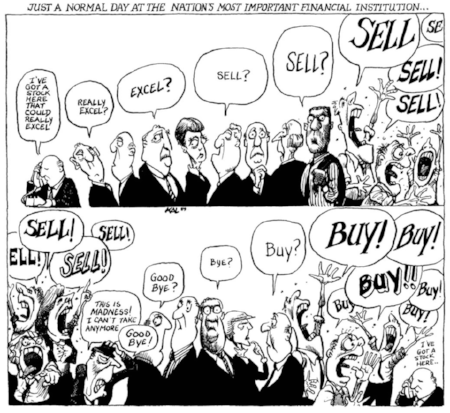
\includegraphics[width=.6\textwidth]{img/ch-investing/FOMOFUD.png}
    \caption{Fear, Uncertainty and Doubt (FUD) wordt Fear Of Missing Out (FOMO)}
    \label{fig:FOMOFUD}
    \end{figure}
    

    